%=======================================================================
%  PLANTILLA DE INFORME -- Sistemas Dinámicos
%
%  Las cajas en gris e itálica son GUÍAS: explican qué va en cada
%  sección. Borralas a medida que escribís, o poné \guiasfalse en la
%  línea correspondiente para ocultarlas todas antes de entregar.
%=======================================================================
\documentclass[11pt,a4paper]{article}
\usepackage{float}
\usepackage[utf8]{inputenc}
\usepackage[T1]{fontenc}
\IfFileExists{spanish.ldf}{\usepackage[spanish,es-noquoting,es-nodecimaldot]{babel}}{}
\usepackage{amsmath,amssymb}
\usepackage{graphicx}
\usepackage{booktabs}
\usepackage{siunitx}
\usepackage[margin=2.5cm]{geometry}
\usepackage{xcolor}
\usepackage{listings}
\usepackage[colorlinks=true,allcolors=blue]{hyperref}

\renewcommand{\abstractname}{Resumen}

\newif\ifguias
\guiasfalse        % <-- cambiar a \guiasfalse para ocultar las guías
\newcommand{\guia}[1]{\ifguias\par\noindent
  {\color{gray!85!black}\small\itshape #1}\par\medskip\fi}

\lstset{basicstyle=\ttfamily\footnotesize,frame=single,framesep=4pt,
        backgroundcolor=\color{black!4},breaklines=true,
        columns=fullflexible,showstringspaces=false}

\sisetup{output-decimal-marker={,},per-mode=symbol}
\DeclareSIUnit{\anio}{a}   % símbolo SI para año

%=======================================================================
\title{\textbf{Trabajo Práctico: competencia interespecífica y control
poblacional de ungulados exóticos}\\[2pt]
       \large Dinámica de Sistemas (I300)}

\author{Agustina Victoria Barrena\\
        \small \texttt{abarrena@udesa.edu.ar}
        \and
        Abril Diaco\\
        \small \texttt{adiaco@udesa.edu.ar}
        \and
        Pilar Otero\\
        \small \texttt{potero@udesa.edu.ar}}

\date{\today}

\begin{document}
\maketitle

%=======================================================================
\begin{abstract}
\guia{El resumen tiene entre 150 y 200 palabras y se escribe AL FINAL.
Cinco oraciones alcanzan: (1) contexto y problema; (2) objetivo concreto
de este trabajo; (3) qué se hizo (datos y método, en una línea);
(4) el resultado principal CON NÚMEROS; (5) qué se concluye.
No lleva citas, ni figuras, ni siglas sin definir. Escribir sólo
``en este trabajo se estudia\dots'' no sirve: eso no dice cuál fue el
resultado.}

El control de una especie invasora en un área con competencia interespecífica no
siempre reduce el impacto ecológico esperado, ya que puede liberar a la especie
competidora de parte de la presión sobre los recursos compartidos. Este trabajo
estima los parámetros de un modelo de Lotka--Volterra de competencia entre el ciervo
axis y el chancho salvaje a partir de censos anuales, y evalúa cómo distintas
políticas de control realimentado sobre el chancho afectan a ambas poblaciones. Los
parámetros se ajustaron por mínimos cuadrados lineales sobre la tasa de crecimiento
per cápita, usando 33 años de datos sintéticos (1992--2024), y el sistema controlado
se simuló bajo leyes de extracción proporcionales y con umbral. El ajuste, validado
con un error relativo medio de 3--4\,\% fuera de muestra, arrojó capacidades de carga
de $K_1\approx1900$ ciervos y $K_2\approx910$ chanchos, con un equilibrio interior
estable en $(x^*,y^*)\approx(1010,540)$; bajo control del chancho, la población de
ciervos aumentó entre un 54\,\% y un 92\,\% a 40 años respecto del escenario sin
control. Estos resultados reproducen, en un modelo simplificado, el mismo efecto de
liberación competitiva observado en el Parque Nacional El Palmar, y muestran que toda
política de manejo realimentada sobre el chancho conlleva un costo colateral
significativo sobre el ciervo.


\medskip
\noindent\textbf{Palabras clave:} competencia interespecífica, modelo de Lotka--Volterra, control realimentado, especies invasoras, estimación de parámetros.

\end{abstract}

%=======================================================================
\section{Introducción}
\label{sec:intro}

% \guia{Cuatro párrafos, en este orden:
% (1) el problema general y por qué importa;
% (2) qué se sabe hasta ahora, con citas \cite{gurtler2018};
% (3) qué falta o qué se quiere responder acá --- el objetivo, enunciado
% de manera verificable;
% (4) cómo está organizado el resto del informe.
% El error típico es escribir toda la teoría en la introducción: la teoría
% va en la Sección~\ref{sec:modelo}.}

En un ecosistema, controlar una especie invasora no siempre produce un efecto aislado ni predecible. Cuando dos poblaciones compiten por alimento, espacio u otros recursos, reducir la abundancia de una de ellas puede liberar a la otra de parte de esa competencia. Así, una medida de manejo pensada para disminuir el impacto de una especie puede modificar indirectamente la dinámica de otra. Este tipo de respuesta es especialmente relevante en áreas protegidas, donde las decisiones de control buscan conservar especies nativas y procesos ecológicos, pero deben tomarse sobre sistemas con múltiples interacciones.

Un ejemplo de este problema aparece en el Parque Nacional El Palmar, donde conviven ungulados exóticos como el ciervo axis (\emph{Axis axis}) y el jabalí o chancho salvaje (\emph{Sus scrofa}). Ambas especies utilizan recursos similares, incluyendo pastos, frutos de palmera y renovales. Estudios realizados en el área mostraron que, luego de implementar controles sobre jabalíes, su abundancia disminuyó, mientras que la población de ciervos axis aumentó marcadamente en los años siguientes \cite{gurtler2018}. Este comportamiento sugiere una interacción competitiva asimétrica: al reducirse una especie, la otra puede experimentar una ventaja indirecta.

En este trabajo se estudia una versión simplificada de ese fenómeno mediante un modelo de Lotka--Volterra de competencia entre dos especies. A partir de datos sintéticos de censos anuales de ciervos y chanchos, el objetivo es estimar los parámetros del modelo, estudiar los equilibrios del sistema y simular la evolución de las poblaciones bajo distintas políticas de control aplicadas sobre los chanchos. El objetivo principal es entender cómo la interacción competitiva entre ambas especies afecta el resultado de una intervención de manejo y, en particular, cuantificar qué ocurre con la población de ciervos cuando se reduce la población de chanchos.

El informe se organiza de la siguiente manera. En la Sección~\ref{sec:modelo} se presentan el modelo utilizado, sus variables y los datos disponibles. En la Sección~\ref{sec:metodos} se describe el procedimiento usado para estimar los parámetros y realizar las simulaciones. En la Sección~\ref{sec:resultados} se muestran los resultados del ajuste, el análisis cualitativo del sistema y los escenarios de control. Finalmente, en las Secciones~\ref{sec:discusion} y~\ref{sec:conclusiones} se interpretan los resultados obtenidos y se resumen las principales conclusiones.

%=======================================================================
\section{Modelo y datos}
\label{sec:modelo}

\subsection{Modelo}
% \guia{Presentar las ecuaciones, definir CADA símbolo con sus unidades e
% indicar las hipótesis que se están asumiendo (por ejemplo: poblaciones
% bien mezcladas, ausencia de estructura etaria, parámetros constantes en
% el tiempo). Numerar sólo las ecuaciones que después se citan.}

Para representar la interacción entre las dos especies se utilizó un modelo de Lotka--Volterra de competencia. Se denota por $x(t)$ la abundancia de ciervos axis y por $y(t)$ la abundancia de chanchos, ambas medidas en individuos. La variable $t$ representa el tiempo medido en años. El modelo sin control está dado por

\begin{equation}
\label{eq:modelo}
\dot x = x\,(a_1 - b_{11}x - b_{12}y), \qquad
\dot y = y\,(a_2 - b_{21}x - b_{22}y),
\end{equation}

donde $a_1$ y $a_2$ son las tasas de crecimiento propias de ciervos y chanchos, respectivamente, y tienen unidades de $1/\text{año}$. Los parámetros $b_{11}$ y $b_{22}$ describen la competencia dentro de cada especie: a medida que hay más individuos de una misma población, su crecimiento se frena por la competencia por recursos. En cambio, $b_{12}$ y $b_{21}$ describen la competencia entre especies: $b_{12}$ mide el efecto de los chanchos sobre los ciervos, y $b_{21}$ el efecto de los ciervos sobre los chanchos. Todos los coeficientes $b_{ij}$ tienen unidades de $1/(\text{año}\cdot\text{individuo})$.

Para interpretar los resultados también se usa la parametrización ecológica equivalente,

\begin{equation}
\label{eq:modelo-ecologico}
\dot x = r_1 x \left(1 - \frac{x + \alpha_{12}y}{K_1}\right), \qquad
\dot y = r_2 y \left(1 - \frac{y + \alpha_{21}x}{K_2}\right).
\end{equation}

En esta forma, $r_1$ y $r_2$ representan las tasas de crecimiento de cada especie, con unidades de $1/\text{año}$. Los parámetros $K_1$ y $K_2$ son las capacidades de carga, es decir, las poblaciones máximas que podrían sostenerse si la otra especie no estuviera presente; se miden en individuos. Los coeficientes $\alpha_{12}$ y $\alpha_{21}$ no tienen unidades y permiten comparar la fuerza de la competencia entre especies. Por ejemplo, $\alpha_{12}$ indica cuánto pesa un chancho, en términos de competencia, sobre la población de ciervos. De manera análoga, $\alpha_{21}$ indica cuánto pesa un ciervo sobre la población de chanchos.

Las relaciones entre ambas parametrizaciones son
\begin{equation}
\label{eq:relaciones-parametros}
r_1 = a_1, \qquad r_2 = a_2, \qquad
K_1 = \frac{a_1}{b_{11}}, \qquad K_2 = \frac{a_2}{b_{22}}, \qquad
\alpha_{12} = \frac{b_{12}}{b_{11}}, \qquad
\alpha_{21} = \frac{b_{21}}{b_{22}}.
\end{equation}

La forma~\eqref{eq:modelo} es la conveniente para \emph{estimar} porque es
lineal en sus seis parámetros: al dividir por la población, la tasa de
crecimiento per cápita queda como una combinación lineal de $1$, $x$ e $y$
(Sección~\ref{sec:metodos}), y el ajuste se reduce a mínimos cuadrados
lineales, con solución única y sin necesidad de valores iniciales. En la
forma~\eqref{eq:modelo-ecologico}, en cambio, los parámetros aparecen
multiplicados y divididos entre sí ($r_1/K_1$, $r_1\alpha_{12}/K_1$), por lo
que estimarlos directamente sería un problema no lineal. A la inversa,
\eqref{eq:modelo-ecologico} es la conveniente para \emph{interpretar}: $K_i$
se mide en individuos y se compara directamente con los censos, y
$\alpha_{ij}$ es adimensional y compara la competencia entre especies con la
competencia dentro de la especie, mientras que los $b_{ij}$, en
$1/(\text{año}\cdot\text{individuo})$, no tienen una lectura ecológica
inmediata.

Más adelante se analiza también el efecto de aplicar una extracción sobre la población de chanchos. Para eso se incorpora una variable de control $u(t)$, medida en individuos por año, que representa la cantidad de chanchos removidos por unidad de tiempo. El modelo controlado queda

\begin{equation}
\label{eq:modelo-control}
\dot x = x\,(a_1 - b_{11}x - b_{12}y), \qquad
\dot y = y\,(a_2 - b_{21}x - b_{22}y) - u(t).
\end{equation}

El modelo toma a cada población como un conjunto homogéneo dentro del área de estudio. Es decir, no distingue zonas del parque, edades ni diferencias entre individuos de una misma especie. Además, se asume que los parámetros no cambian con el tiempo. Estas simplificaciones permiten enfocarse en lo central del trabajo: la competencia entre ciervos y chanchos, y qué ocurre cuando se controla solamente a los chanchos.

\subsection{Datos}
% \guia{Origen, período cubierto, frecuencia de muestreo, número de
% observaciones, unidades y --- importante --- qué se sabe del error de
% medición. Si los datos son sintéticos, decirlo acá de forma explícita.}

Para ajustar el modelo se trabajó con una serie anual de abundancias de ciervos axis y chanchos en el área de estudio. Los datos cubren el período 1992-2024, con un censo por año, lo que da un total de $N=33$ observaciones para cada especie. En todos los casos, las cantidades están expresadas como número de individuos.

La serie utilizada fue provista junto con la consigna y es importante aclarar que no corresponde a censos reales. Se trata de datos sintéticos, generados a partir de un modelo y luego modificados con ruido de observación. De todos modos, los órdenes de magnitud fueron elegidos para ser compatibles con valores reportados en estudios sobre el caso del Parque Nacional El Palmar.

Según la información provista, el error de medición de las abundancias es aproximadamente del 5\%. Además, este error puede pensarse como multiplicativo: no afecta tanto como una cantidad fija de individuos, sino como una proporción del valor observado. Por eso, una forma razonable de interpretarlo es como ruido \textit{lognormal} sobre las abundancias.

%=======================================================================
\section{Métodos}
\label{sec:metodos}

% \guia{Un tercero tiene que poder reproducir los resultados leyendo esta
% sección. Va en pasado o en impersonal, no en imperativo (``se estimaron
% los parámetros'', no ``estimar los parámetros''). Se describe el método,
% no el código: se dice ``mínimos cuadrados no lineales con el algoritmo
% de Levenberg--Marquardt'', no ``se usó \texttt{least\_squares}''.
% Incluir: el método de estimación, el integrador numérico y sus
% tolerancias, el criterio de validación y cómo se cuantificó la
% incertidumbre.}

La estimación de parámetros se hizo aprovechando que el modelo puede escribirse de forma lineal si se trabaja con tasas de crecimiento per cápita. Para eso, se dividió cada ecuación de \eqref{eq:modelo} por la población correspondiente. Así se obtuvo

\begin{equation}
\label{eq:log-derivadas}
\frac{d}{dt}\ln x(t) = a_1 - b_{11}x(t) - b_{12}y(t), \qquad
\frac{d}{dt}\ln y(t) = a_2 - b_{21}x(t) - b_{22}y(t).
\end{equation}

Como los datos son anuales, la derivada de los logaritmos se aproximó con diferencias entre observaciones consecutivas. Además, las abundancias que aparecen en el lado derecho se evaluaron en el punto medio del intervalo:

\[
\frac{d}{dt}\ln x(t_{k+1/2})
\simeq
\frac{\ln x_{k+1}-\ln x_k}{t_{k+1}-t_k},
\qquad
x_{k+1/2}=\frac{x_k+x_{k+1}}{2},
\qquad
y_{k+1/2}=\frac{y_k+y_{k+1}}{2}.
\]

Con estas cantidades se armó, para cada especie, un sistema sobredeterminado
$A\theta\approx g$ con una fila por intervalo entre censos ($k=1,\dots,32$):
\[
A=\begin{pmatrix}
1 & -x_{1+1/2} & -y_{1+1/2}\\
\vdots & \vdots & \vdots\\
1 & -x_{32+1/2} & -y_{32+1/2}
\end{pmatrix},\quad
\theta_x=\begin{pmatrix}a_1\\ b_{11}\\ b_{12}\end{pmatrix},\quad
\theta_y=\begin{pmatrix}a_2\\ b_{21}\\ b_{22}\end{pmatrix},\quad
g_x=\begin{pmatrix}g_{x,1+1/2}\\ \vdots\\ g_{x,32+1/2}\end{pmatrix},
\]
donde $g_{x,k+1/2}=(\ln x_{k+1}-\ln x_k)/\Delta t$ es la tasa de crecimiento
per cápita aproximada de los ciervos, y $g_y$ se define de forma análoga con
$y$. Ambas especies comparten la misma matriz $A\in\mathbb{R}^{32\times3}$;
se resolvieron por separado $A\theta_x\approx g_x$ y $A\theta_y\approx g_y$,
minimizando $\|A\theta-g\|_2^2$ mediante descomposición en valores
singulares.


Además del ajuste con datos anuales, se repitió el procedimiento usando una observación cada dos años. Esta comparación permite ver el compromiso entre el error de aproximación de la derivada y la amplificación del ruido de medición al calcular diferencias entre observaciones cercanas.

Para validar el modelo fuera de muestra, se estimaron los parámetros usando únicamente los datos entre 1992 y 2012. Luego se tomó como condición inicial el estado observado en 2012 y se simuló el sistema hasta 2024. Las predicciones para el período 2013--2024 se compararon con los datos reservados mediante el error relativo medio, calculado por separado para ciervos y chanchos:

\[
\text{error relativo medio}
=
\frac{1}{N}\sum_k
\left|
\frac{\hat z_k-z_k}{z_k}
\right|.
\]

La estabilidad de cada equilibrio se determinó linealizando el
sistema~\eqref{eq:modelo}: se evaluó el jacobiano
\[
J(x,y)=\begin{pmatrix}
a_1-2b_{11}x-b_{12}y & -b_{12}x\\
-b_{21}y & a_2-b_{21}x-2b_{22}y
\end{pmatrix}
\]
en cada punto y se lo clasificó según su traza, su determinante y sus
autovalores.

Las simulaciones se realizaron con un integrador Runge--Kutta explícito de
paso adaptativo de órdenes 4 y 5 (Dormand--Prince), con tolerancias relativa
y absoluta de $10^{-8}$. Para la validación se integró desde 2012 hasta 2024,
y para la proyección sin control, desde 2024 hasta 2060. En los escenarios de
control se simularon 40 años a partir del estado observado en 2024, y además
se calcularon analíticamente los equilibrios del sistema controlado para
distinguir el estado a 40 años del régimen permanente.


Para estudiar el efecto del manejo se consideraron tres políticas de extracción de chanchos. Primero se simuló una extracción proporcional a la abundancia, $u(t)=ky(t)$, con $k=0$, $0{,}1$, $0{,}2$ y $0{,}4$. Luego se incorporó una saturación en la extracción, $u(t)=\min\{u_{\max},ky(t)\}$, con $u_{\max}=120$ individuos/año. Por último, se analizó una política con umbral,

\[
u(t)=\min\{u_{\max},k\max(0,y(t)-y_{\mathrm{ref}})\},
\]

tomando $y_{\mathrm{ref}}=150$ individuos y probando $k=0{,}3$, $0{,}5$, $1{,}0$ y $2{,}0$. En cada caso se registró la evolución de ambas poblaciones y el total de chanchos extraídos, calculado como la integral temporal de $u(t)$.

Para cuantificar la incertidumbre de los seis parámetros y de las cantidades
derivadas ($K_1$, $K_2$, $\alpha_{12}$, $\alpha_{21}$) se aplicó un bootstrap
no paramétrico sobre los pares $(A_k,g_k)$ del sistema de mínimos cuadrados:
se generaron $200$ réplicas remuestreando con reemplazo los $32$ intervalos
disponibles (semilla fija), y el intervalo de confianza del 95\,\% de cada
parámetro se tomó como los percentiles 2,5 y 97,5 de su distribución
empírica. Además, para evaluar la influencia del censo de 1992, que tiene la
menor abundancia de ciervos de la serie, se repitió el ajuste excluyendo ese
año.


%=======================================================================
\section{Resultados}
\label{sec:resultados}

\guia{Sólo hechos: qué dio. La interpretación va en la Discusión.
Cada resultado numérico con su incertidumbre y sus unidades. Cada figura
y cada tabla tiene que estar mencionada en el texto (``la
Figura~\ref{fig:ajuste} muestra\dots''); si una figura no se menciona,
sobra.}

\subsection{Estimación de parámetros}
\label{sec:estim}
Al realizar el ajuste por mínimos cuadrados descrito en la
Sección~\ref{sec:metodos}, utilizando la serie anual completa
(1992--2024), se obtuvieron los seis parámetros del modelo~\eqref{eq:modelo}
que se reportan en la Tabla~\ref{tab:parametros}. A partir de ellos,
mediante las relaciones~\eqref{eq:relaciones-parametros}, se obtuvieron las
capacidades de carga $K_1$ y $K_2$ y los coeficientes de competencia
relativa $\alpha_{12}$ y $\alpha_{21}$. Los intervalos de confianza del
95\,\% se estimaron por bootstrap sobre las filas del sistema lineal.

\begin{table}[H]
\centering
\caption{Parámetros del modelo~\eqref{eq:modelo} estimados por mínimos
cuadrados lineales sobre la serie anual 1992--2024, con sus unidades. La
parte inferior reúne las cantidades derivadas
mediante~\eqref{eq:relaciones-parametros}. El IC 95\,\% corresponde a los
percentiles 2,5 y 97,5 de 200 réplicas de bootstrap. Los coeficientes
$b_{ij}$ y su intervalo están expresados en unidades de
$10^{-4}$.}
\label{tab:parametros}
\begin{tabular}{lccc}
\toprule
Parámetro & Unidad & Estimación & IC 95\,\% \\
\midrule
$a_1$ & $1/\text{año}$ & $0{,}450$ & $[-0{,}070,\ 0{,}563]$ \\
$a_2$ & $1/\text{año}$ & $0{,}638$ & $[\phantom{-}0{,}298,\ 0{,}997]$ \\
$b_{11}$ & $10^{-4}/(\text{año}\cdot\text{ind})$ & $2{,}35$ & $[\phantom{-}0{,}73,\ 3{,}20]$ \\
$b_{12}$ & $10^{-4}/(\text{año}\cdot\text{ind})$ & $3{,}93$ & $[-2{,}42,\ 6{,}03]$ \\
$b_{21}$ & $10^{-4}/(\text{año}\cdot\text{ind})$ & $2{,}55$ & $[\phantom{-}1{,}16,\ 4{,}11]$ \\
$b_{22}$ & $10^{-4}/(\text{año}\cdot\text{ind})$ & $7{,}02$ & $[\phantom{-}2{,}90,\ 11{,}6]$ \\
\midrule
$K_1$        & individuos & $1914$ & $[-769,\ 2821]$ \\
$K_2$        & individuos & $909$  & $[\phantom{-}796,\ 1119]$ \\
$\alpha_{12}$ & ---       & $1{,}67$ & $[-2{,}65,\ 3{,}10]$ \\
$\alpha_{21}$ & ---       & $0{,}36$ & $[\phantom{-}0{,}18,\ 0{,}66]$ \\
\bottomrule
\end{tabular}
\end{table}

Los parámetros asociados a los ciervos ($a_1$, $b_{12}$, $K_1$ y
$\alpha_{12}$) presentan intervalos anchos que incluyen valores
negativos, mientras que los asociados a los chanchos ($a_2$, $b_{21}$,
$b_{22}$, $K_2$ y $\alpha_{21}$) resultan más acotados y de signo
positivo.

Al repetir el ajuste excluyendo el censo de 1992, los parámetros de los
ciervos cambian fuertemente: $a_1$ pasa de $0{,}45$ a $0{,}28$~$1/\text{año}$,
$K_1$ de $1900$ a $1500$ individuos y $\alpha_{12}$ de $1{,}67$ a $1{,}00$.
Los de los chanchos cambian menos: $K_2$ varía un $2\,\%$ y $\alpha_{21}$,
un $8\,\%$.

Para analizar la calidad del ajuste, la Figura~\ref{fig:residuos} muestra
los residuos, la tasa de crecimiento per cápita observada menos la
predicha, para cada especie en función del tiempo.

\begin{figure}[H]
\centering
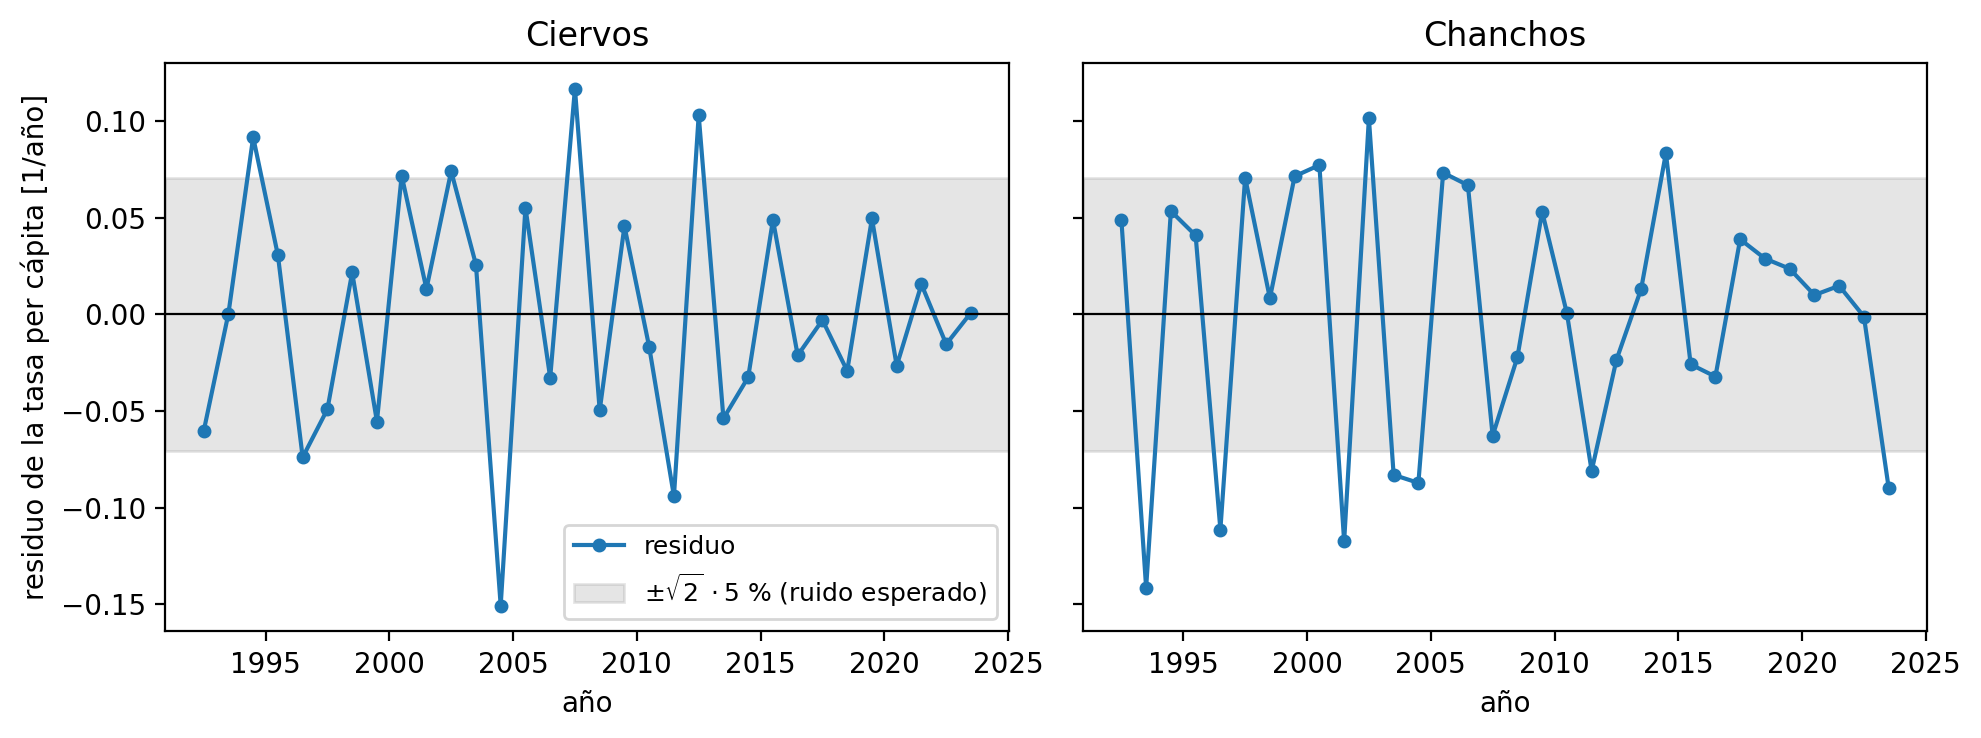
\includegraphics[width=\linewidth]{residuos.png}
\caption{Residuos del ajuste lineal (tasa de crecimiento per cápita
observada menos la predicha por~\eqref{eq:log-derivadas}), en
$1/\text{año}$, para ciervos (izquierda) y chanchos (derecha). La banda
gris indica $\pm\sqrt{2}\cdot 0{,}05\approx\pm0{,}071$~$1/\text{año}$, la
dispersión esperada sólo por el error de censo del 5\,\%.}
\label{fig:residuos}
\end{figure}

El desvío estándar de los residuos es de $0{,}062$~$1/\text{año}$ para los
ciervos y de $0{,}069$~$1/\text{año}$ para los chanchos, similar al valor
$\sqrt{2}\cdot0{,}05\approx0{,}071$~$1/\text{año}$ que se espera sólo por el
error de censo. La Tabla~\ref{tab:submuestreo} compara este ajuste con el
obtenido usando un censo de cada dos ($\Delta t=2$ años): el desvío de los
residuos se reduce a la mitad, de acuerdo con la amplificación del ruido como
$1/\Delta t$, y los parámetros cambian entre un $2\,\%$ y un $24\,\%$.

\begin{table}[H]
\centering
\caption{Comparación entre el ajuste con todos los censos ($\Delta t=1$~año,
32 intervalos) y con un censo de cada dos ($\Delta t=2$~años, 16
intervalos). $\sigma_{\text{res}}$ es el desvío estándar de los residuos y
$\sigma_{\text{ruido}}=\sqrt{2}\cdot0{,}05/\Delta t$, el esperado sólo por
el error de censo.}
\label{tab:submuestreo}
\begin{tabular}{lcc}
\toprule
 & $\Delta t=1$~año & $\Delta t=2$~años \\
\midrule
$a_1$ [$1/\text{año}$] & $0{,}45$ & $0{,}51$ \\
$a_2$ [$1/\text{año}$] & $0{,}64$ & $0{,}70$ \\
$K_1$ [individuos] & $1900$ & $2200$ \\
$K_2$ [individuos] & $910$ & $880$ \\
$\alpha_{12}$ & $1{,}67$ & $2{,}07$ \\
$\alpha_{21}$ & $0{,}36$ & $0{,}31$ \\
\midrule
$\sigma_{\text{res}}$ ciervos / chanchos [$1/\text{año}$] & $0{,}062$ / $0{,}069$ & $0{,}035$ / $0{,}036$ \\
$\sigma_{\text{ruido}}$ [$1/\text{año}$] & $0{,}071$ & $0{,}035$ \\
\bottomrule
\end{tabular}
\end{table}

Como última verificación se realizó una validación fuera de muestra donde se
reestimaron los parámetros usando sólo los datos de 1992--2012 y, tomando
ese último año como punto de partida, se simuló la evolución del sistema
hasta 2024. Las predicciones para el período reservado 2013--2024 se
compararon con los datos observados, obteniendo  un error relativo medio de
$3{,}2\,\%$ para los ciervos y $3{,}9\,\%$ para los chanchos.

\subsection{Análisis cualitativo}
\label{sec:cualitativo}

El sistema~\eqref{eq:modelo} admite cuatro equilibrios. Anulando $\dot x$ y
$\dot y$ se obtienen la extinción total $(0,0)$, los estados con una sola
especie $(K_1,0)$ y $(0,K_2)$, y un equilibrio interior $(x^\ast,y^\ast)$
en el que ambas poblaciones son no nulas. Este último resuelve el sistema
lineal $b_{11}x+b_{12}y=a_1$, $b_{21}x+b_{22}y=a_2$, cuya solución por la
regla de Cramer es

\begin{equation}
\label{eq:interior}
x^\ast=\frac{a_1 b_{22}-a_2 b_{12}}{b_{11}b_{22}-b_{12}b_{21}},
\qquad
y^\ast=\frac{a_2 b_{11}-a_1 b_{21}}{b_{11}b_{22}-b_{12}b_{21}}.
\end{equation}

Evaluados con los parámetros de la Tabla~\ref{tab:parametros}, los cuatro
equilibrios toman los valores de la Tabla~\ref{tab:equilibrios}, junto con
los autovalores del jacobiano en cada uno. El origen es un nodo inestable,
los dos equilibrios con una sola especie son sillas y el equilibrio interior,
con ambas coordenadas positivas, es un nodo estable. Sus autovalores
corresponden a constantes de tiempo de $1{,}8$ y $15{,}6$ años. Las
condiciones de coexistencia se cumplen: $K_1\approx1900>\alpha_{12}K_2\approx1500$
y $K_2\approx910>\alpha_{21}K_1\approx700$.

\begin{table}[H]
\centering
\caption{Equilibrios del sistema~\eqref{eq:modelo} evaluados con los
parámetros estimados, autovalores del jacobiano en cada uno y su
clasificación.}
\label{tab:equilibrios}
\begin{tabular}{lcccc}
\toprule
Equilibrio & $(x,\,y)$ [individuos] & $\lambda_1$ [$1/\text{año}$] & $\lambda_2$ [$1/\text{año}$] & Tipo \\
\midrule
$(0,0)$                    & $(0,\,0)$      & $0{,}45$   & $0{,}64$  & nodo inestable \\
$(K_1,0)$                  & $(1914,\,0)$   & $-0{,}45$  & $0{,}15$  & silla \\
$(0,K_2)$                  & $(0,\,909)$    & $-0{,}64$  & $0{,}094$ & silla \\
Interior $(x^\ast,y^\ast)$ & $(1010,\,542)$ & $-0{,}064$ & $-0{,}55$ & nodo estable \\
\bottomrule
\end{tabular}
\end{table}

La Figura~\ref{fig:fases} muestra el diagrama de fases: las nulclinas no
triviales se cortan en el primer cuadrante, en el equilibrio interior, y la
trayectoria de los censos avanza hacia él junto a la nulclina $\dot y=0$.

\begin{figure}[H]
\centering
\begin{minipage}[t]{0.49\linewidth}
\centering
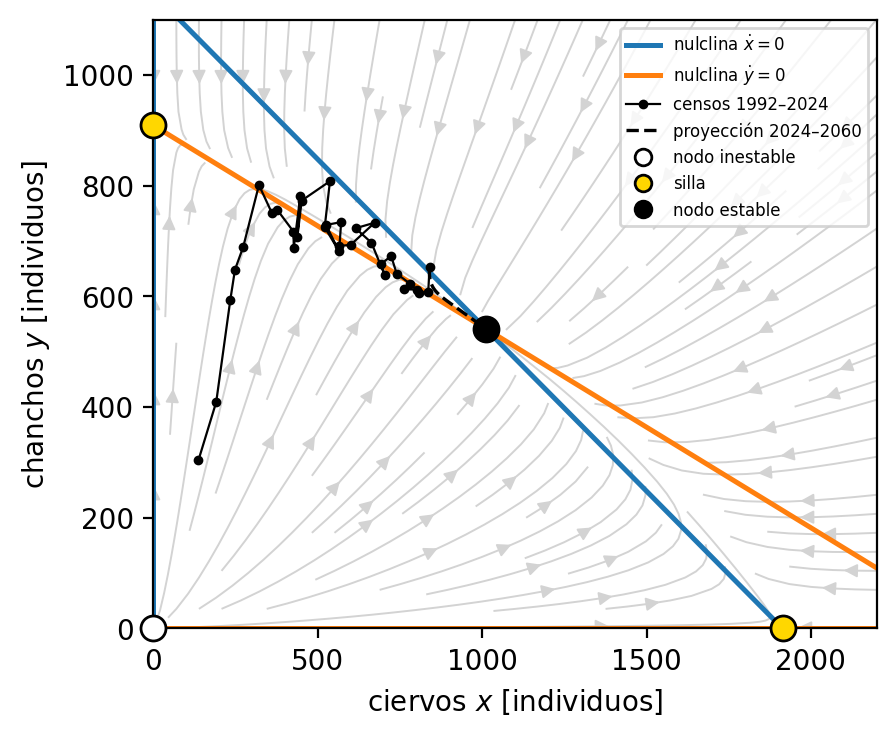
\includegraphics[width=\linewidth]{fases.png}
\caption{Diagrama de fases del modelo~\eqref{eq:modelo} con los parámetros
estimados: campo de direcciones (gris), nulclinas $\dot x=0$ (azul) y
$\dot y=0$ (naranja), equilibrios clasificados según su tipo, trayectoria de
los censos 1992--2024 y proyección entre 2024 y 2060. Ejes en individuos.}
\label{fig:fases}
\end{minipage}\hfill
\begin{minipage}[t]{0.49\linewidth}
\centering
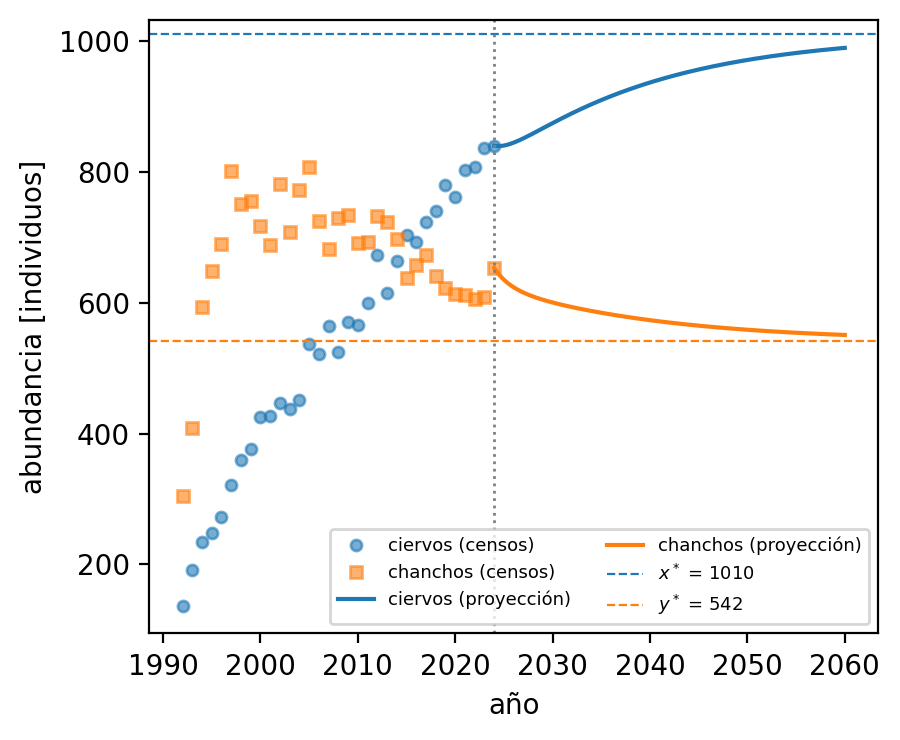
\includegraphics[width=\linewidth]{proyeccion.png}
\caption{Censos 1992--2024 (puntos) y proyección del
modelo~\eqref{eq:modelo} sin control entre 2024 y 2060 (líneas) desde el
estado observado en 2024, en individuos. Las líneas discontinuas indican
$x^\ast$ e $y^\ast$.}
\label{fig:proyeccion}
\end{minipage}
\end{figure}

El sistema no había alcanzado el equilibrio en 2024. El estado observado ese
año, $(x,y)=(840,\,653)$ individuos, tiene a los ciervos $170$ individuos por
debajo de $x^\ast$ y a los chanchos $111$ por encima de $y^\ast$, es decir, a
una distancia relativa
$\sqrt{(\Delta x/x^\ast)^2+(\Delta y/y^\ast)^2}\approx27\,\%$ del equilibrio
interior $(1010,\,542)$. Al integrar el modelo~\eqref{eq:modelo} sin control
desde ese estado (Figura~\ref{fig:proyeccion}), la trayectoria se acerca al
equilibrio y queda a menos del $5\,\%$ de él recién hacia 2050. En 2060, el
estado proyectado es $(989,\,551)$ individuos.

\subsection{Efecto del control}
\label{sec:control}

Se simuló la evolución del sistema~\eqref{eq:modelo-control} durante 40 años
desde el estado observado en 2024, bajo una extracción proporcional a la
abundancia de chanchos, $u(t)=k\,y(t)$, con $k\in\{0,\,0{,}1,\,0{,}2,\,0{,}4\}$.
La Figura~\ref{fig:control} muestra la evolución de ambas poblaciones y del
esfuerzo de extracción $u(t)$.

\begin{figure}[H]
\centering
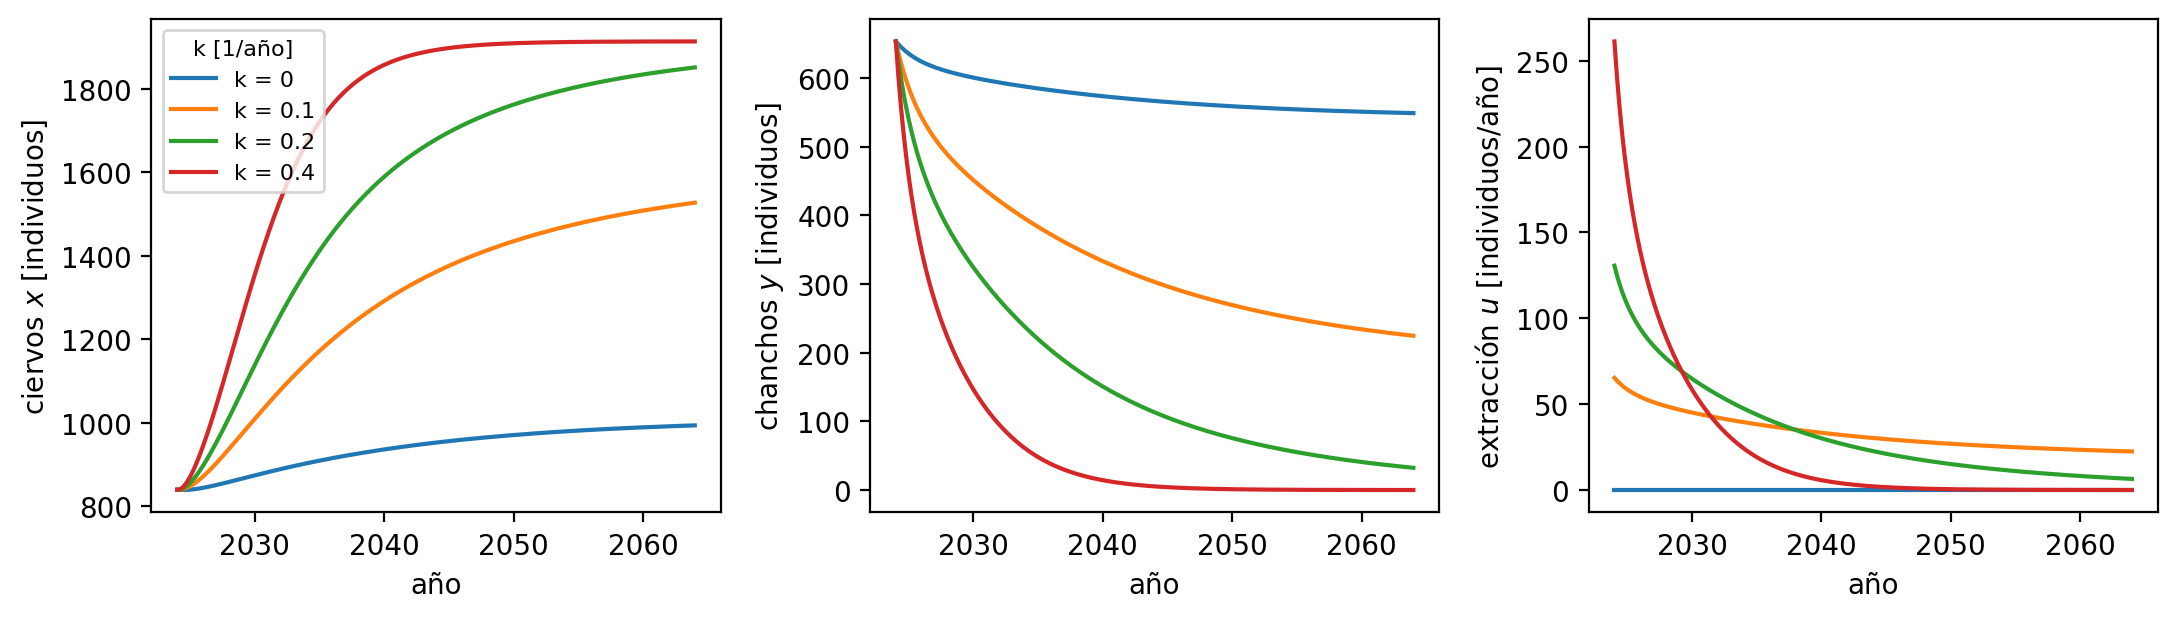
\includegraphics[width=\linewidth]{simulaciones.png}
\caption{Extracción proporcional $u=ky$ durante 40 años desde 2024, para
los cuatro valores de $k$ (en $1/\text{año}$). De izquierda a derecha:
población de ciervos $x(t)$ y de chanchos $y(t)$, en individuos, y
extracción $u(t)$, en individuos/año.}
\label{fig:control}
\end{figure}

La Tabla~\ref{tab:control} reporta el estado a 40 años, el equilibrio al que
tiende cada escenario y el total de animales extraídos, calculado como la
integral de $u(t)$ sobre los 40 años. Con $u=ky$, el
sistema~\eqref{eq:modelo-control} es el mismo modelo~\eqref{eq:modelo} con
$a_2$ reemplazado por $a_2-k$. Por lo tanto, los chanchos sobreviven en el
equilibrio sólo si $a_2-k>b_{21}K_1$, es decir, si
\begin{equation}
\label{eq:kcrit}
k<k_c=a_2-b_{21}K_1\approx0{,}15~1/\text{año}.
\end{equation}
El valor $k_c$ coincide con el autovalor positivo de la silla $(K_1,0)$, que
mide la tasa a la que los chanchos pueden invadir una población de ciervos
en su capacidad de carga. Para $k=0{,}1$ el sistema tiende a un nuevo
equilibrio de coexistencia, mientras que para $k=0{,}2$ y $k=0{,}4$ los
chanchos se extinguen. Con $k=0{,}2$, sin embargo, a los 40 años todavía
quedan 32 chanchos, porque la convergencia es lenta.

\begin{table}[H]
\centering
\caption{Extracción proporcional $u=ky$: estado a 40 años, equilibrio al que
tiende el sistema (calculado analíticamente) y total de animales extraídos
en 40 años. $\Delta x$ es el aumento de la población de ciervos a 40 años
respecto del caso sin control ($k=0$). Poblaciones en individuos.}
\label{tab:control}
\begin{tabular}{ccccc}
\toprule
$k$ [$1/\text{año}$] & $(x,\,y)$ a 40 años & $(x,\,y)$ equilibrio & $\Delta x$ [\%] & Extraídos \\
\midrule
$0$     & $(994,\,549)$  & $(1010,\,542)$ & ---   & $0$    \\
$0{,}1$ & $(1528,\,225)$ & $(1614,\,180)$ & $+54$ & $1340$ \\
$0{,}2$ & $(1851,\,32)$  & $(1914,\,0)$   & $+86$ & $1336$ \\
$0{,}4$ & $(1914,\,0)$   & $(1914,\,0)$   & $+92$ & $1001$ \\
\bottomrule
\end{tabular}
\end{table}

Se repitió la simulación incorporando el tope operativo de las partidas de
caza, $u(t)=\min\{u_{\max},\,k\,y(t)\}$ con $u_{\max}=120$ individuos/año.
Se toma como objetivo de la política reducir la población de chanchos y,
para $k>k_c$, llevarla a la extinción. A los 40 años, el estado de ambas
especies resulta idéntico con y sin saturación para los tres valores de $k$
(los de la Tabla~\ref{tab:control}). Lo único que cambia es el total
extraído con $k=0{,}4$: $1019$ chanchos con tope, contra $1001$ sin él. Como
muestra la Figura~\ref{fig:saturacion}, el
tope sólo se alcanza al principio. Con $k=0{,}1$ nunca se alcanza, porque
$ky\le65$ individuos/año. Con $k=0{,}2$ se alcanza durante los primeros
$0{,}4$ años y con $k=0{,}4$, durante los primeros $4$ años. En este último
caso, la trayectoria de los chanchos llega a diferir hasta en $104$
individuos de la del caso sin tope.

\begin{figure}[H]
\centering
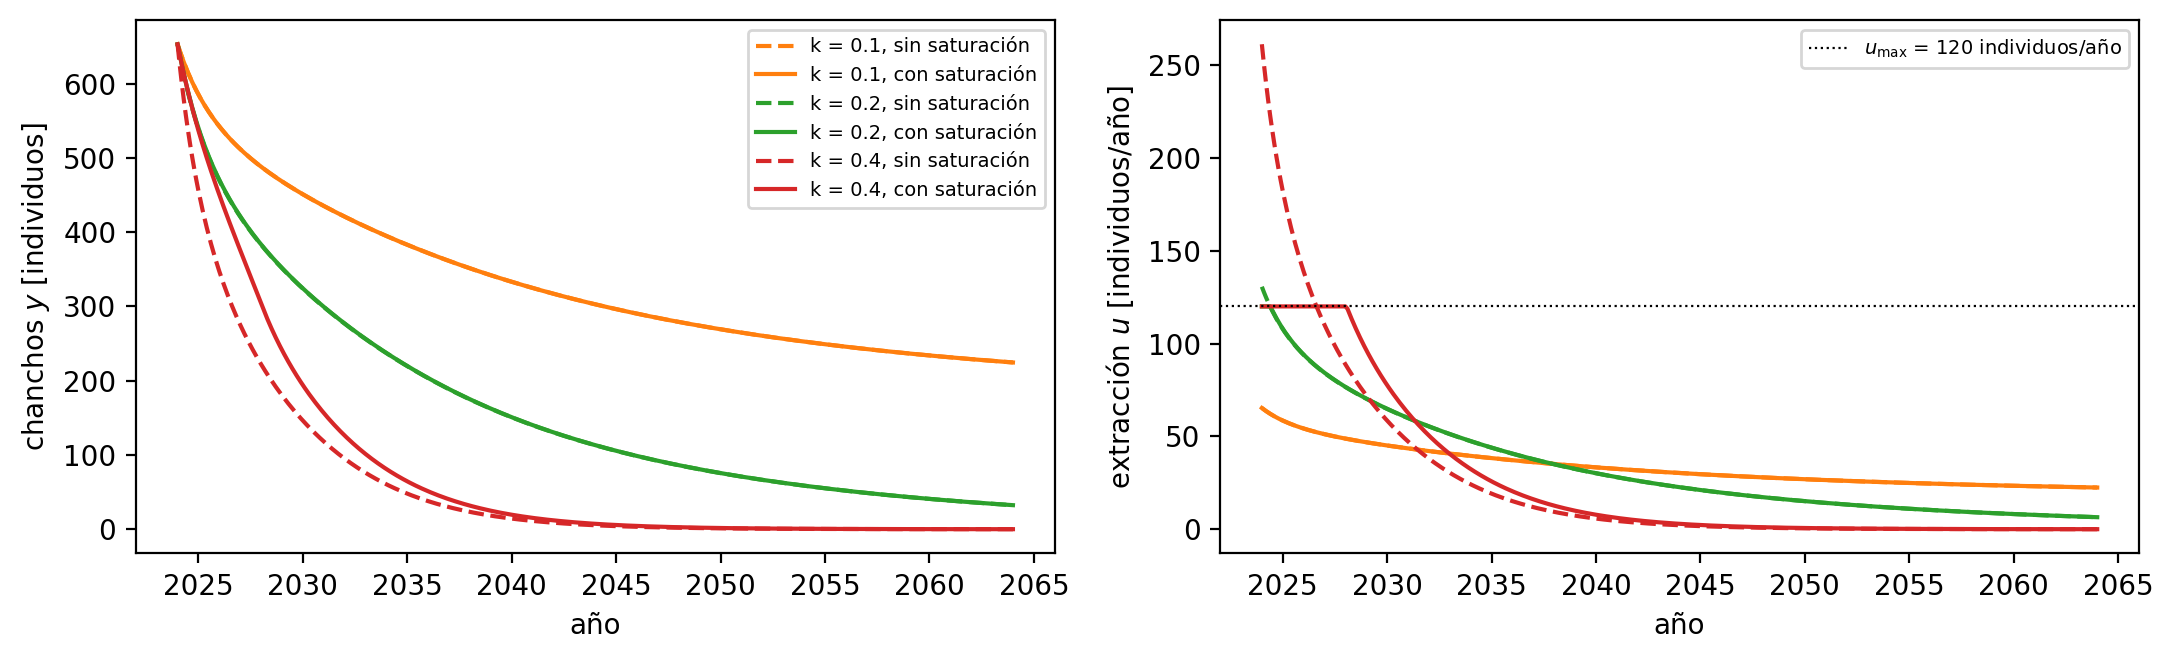
\includegraphics[width=\linewidth]{saturacion.png}
\caption{Población de chanchos $y(t)$ (izquierda) y extracción $u(t)$
(derecha) sin saturación (líneas discontinuas) y con saturación (líneas
continuas), para $k\in\{0{,}1,\,0{,}2,\,0{,}4\}$~$1/\text{año}$. La línea
punteada indica el tope $u_{\max}=120$ individuos/año.}
\label{fig:saturacion}
\end{figure}

Por último se simuló una política que sólo extrae cuando la población supera
un umbral de daño, $u(t)=\min\{u_{\max},\,k\max(0,\,y(t)-y_{\mathrm{ref}})\}$,
con $y_{\mathrm{ref}}=150$ individuos y
$k\in\{0{,}3,\,0{,}5,\,1{,}0,\,2{,}0\}$~$1/\text{año}$. La
Tabla~\ref{tab:umbral} reporta, para cada $k$, la población final de
chanchos, el error de regulación en régimen permanente
$e=y_f-y_{\mathrm{ref}}$, la extracción que se sostiene en régimen
$u_{ss}=k\,e$, el tiempo de establecimiento y la población final de ciervos.
En los cuatro casos, la extracción arranca saturada en $u_{\max}$
(Figura~\ref{fig:umbral}). El error disminuye al aumentar $k$, de $+65$ a
$+8$ individuos, pero se mantiene positivo, mientras que $u_{ss}$ varía poco,
entre $17$ y $19$ individuos/año. Se eligió $k=1{,}0$~$1/\text{año}$ (ver
Sección~\ref{sec:discusion}), con el que la población se estabiliza en $167$
individuos, $17$ por encima del umbral, en unos $10$ años.

\begin{table}[H]
\centering
\small
\caption{Política con umbral ($y_{\mathrm{ref}}=150$ individuos): población
final de chanchos $y_f$, error de regulación en régimen permanente $e$,
extracción en régimen $u_{ss}=k\,e$, tiempo de establecimiento al $5\,\%$
$t_s$, población final de ciervos $x_f$ y su aumento respecto del caso sin
control. Valores a 40 años.}
\label{tab:umbral}
\begin{tabular}{ccccccc}
\toprule
$k$ [$1/\text{año}$] & $y_f$ [ind] & $e$ [ind] & $u_{ss}$ [ind/año] & $t_s$ [años] & $x_f$ [ind] & $\Delta x$ [\%] \\
\midrule
$0{,}3$ & $215$ & $+65$ & $19$ & $21$ & $1555$ & $+56$ \\
$0{,}5$ & $187$ & $+37$ & $18$ & $15$ & $1603$ & $+61$ \\
$1{,}0$ & $167$ & $+17$ & $17$ & $10$ & $1635$ & $+64$ \\
$2{,}0$ & $158$ & $+8$  & $17$ & $7$  & $1650$ & $+66$ \\
\bottomrule
\end{tabular}
\end{table}

\begin{figure}[H]
\centering
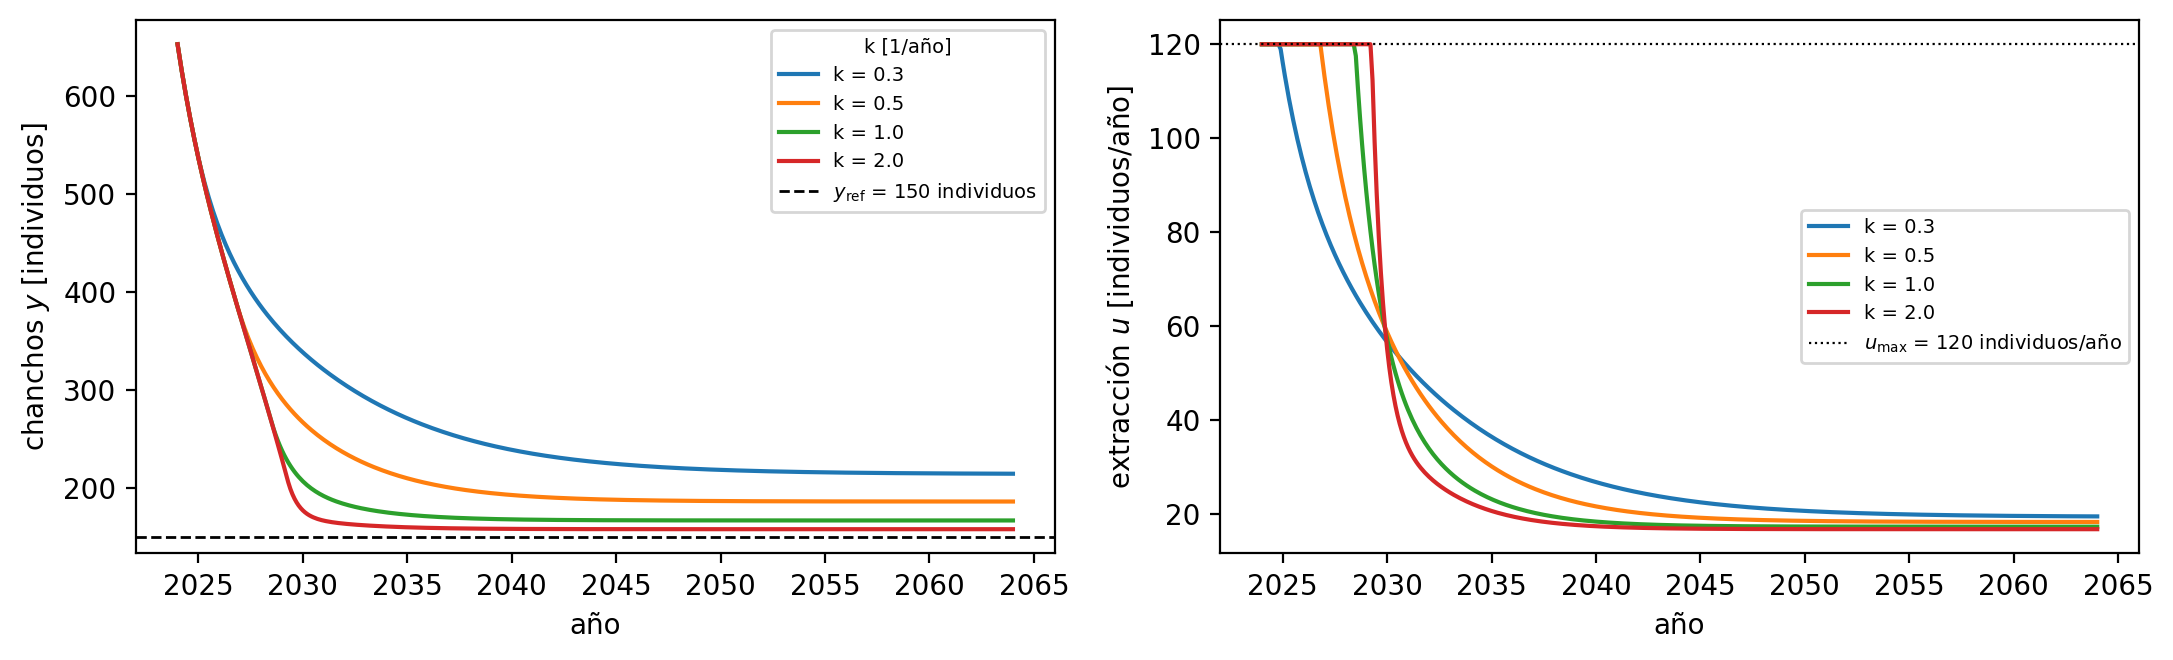
\includegraphics[width=\linewidth]{umbral.png}
\caption{Política con umbral $u=\min\{u_{\max},\,k\max(0,\,y-y_{\mathrm{ref}})\}$
para cuatro valores de $k$. Izquierda: población de chanchos $y(t)$, en
individuos; la línea discontinua marca $y_{\mathrm{ref}}=150$ individuos.
Derecha: extracción $u(t)$, en individuos/año; la línea punteada marca
$u_{\max}=120$ individuos/año.}
\label{fig:umbral}
\end{figure}

En el caso sin control la población de ciervos alcanza $994$ individuos a los
40 años. En todos los escenarios de extracción de chanchos esa población
resulta mayor: entre $+54\,\%$ y $+92\,\%$ bajo extracción proporcional
(Tabla~\ref{tab:control}) y entre $+56\,\%$ y $+66\,\%$ bajo la política con
umbral (Tabla~\ref{tab:umbral}).


%=======================================================================
\section{Discusión}
\label{sec:discusion}


\paragraph{Calidad del ajuste.}
En ambos muestreos el desvío de los residuos coincide con el esperado sólo
por el error de censo (Tabla~\ref{tab:submuestreo}): el error de truncamiento
de la derivada es despreciable frente al ruido, y submuestrear no mejora el
ajuste sino que sólo reduce los datos a la mitad, por lo que se usó
$\Delta t=1$~año. La validación fuera de muestra (errores de $3{,}2$ y
$3{,}9\,\%$, menores que el $5\,\%$ del censo) indica que el modelo captura
la dinámica conjunta, aunque los parámetros de los ciervos quedan mal
determinados: el censo de 1992, con la menor abundancia de la serie, es un
punto de alta influencia, y sin él $\alpha_{12}$ baja de $1{,}67$ a $1{,}00$.

\paragraph{Competencia asimétrica y coexistencia.}
Un ciervo pesa sobre los chanchos apenas un tercio de lo que pesa un chancho
adicional ($\alpha_{21}\approx0{,}36$), mientras que el efecto de un chancho
sobre los ciervos es comparable o mayor al de otro ciervo
($\alpha_{12}\approx1$--$1{,}7$). Lo que sí resulta robusto es que la
competencia dentro de cada especie domina sobre la competencia entre especies
($\alpha_{12}\alpha_{21}\approx0{,}61<1$, y $0{,}34$ sin 1992): las nulclinas
se cortan en el primer cuadrante, los equilibrios con una sola especie son
sillas y el sistema converge a la coexistencia (Figura~\ref{fig:fases}). Es
el caso opuesto a la exclusión competitiva, en la que las nulclinas no se
cortan y sobrevive una sola especie~\cite{murray}. La constante de tiempo
lenta, de $15{,}6$ años, explica que el sistema no estuviera en equilibrio
en 2024 y que 40 años no alcancen para llegar al régimen con $k=0{,}2$.

\paragraph{El control libera a los ciervos.}
En todos los escenarios de control, los ciervos terminan entre un $54$ y un
$92\,\%$ por encima del caso sin control (Tablas~\ref{tab:control}
y~\ref{tab:umbral}): al reducir a su competidor, quedan liberados de parte
de la presión sobre los recursos. Con $k>k_c$ el efecto es máximo, porque los
chanchos se extinguen y los ciervos tienden a su capacidad de carga
$K_1\approx1900$, casi el doble del equilibrio sin control. Además, un
esfuerzo mayor no implica más animales extraídos: con $k=0{,}4$ se extraen
$1001$ chanchos en 40 años, contra $1340$ con $k=0{,}1$, porque la población
colapsa rápido y luego queda poco para extraer.

\paragraph{Saturación y política con umbral.}
La saturación sólo modifica el transitorio: el tope actúa en los primeros
años, cuando $ky$ es grande, mientras que en régimen la extracción necesaria
es menor que $u_{\max}$, por lo que el equilibrio y el objetivo no cambian.
En la política con umbral, el error no nulo es propio de un control
proporcional: en equilibrio hay que seguir extrayendo
$u_{ss}\approx17$--$19$ individuos/año para compensar el crecimiento de los
chanchos, y eso requiere $e=u_{ss}/k>0$. Subir la ganancia del lazo reduce
el error aproximadamente como $1/k$, pero no lo anula. Se eligió $k=1{,}0$
porque también amplifica el error de censo: un $5\,\%$ de error, unos
$\pm8$ chanchos, se traduce en $\pm8k$ individuos/año en la cuota de
extracción. Con $k=2$ eso equivale a $\pm16$ individuos/año, del orden de
$u_{ss}$, mientras que con $k=1$ el error queda en $17$ individuos ($11\,\%$
de $y_{\mathrm{ref}}$) y la población se estabiliza en unos 10 años.

\paragraph{Limitaciones y comparación con el caso real.}
El modelo supone poblaciones homogéneas, sin estructura espacial ni etaria,
parámetros constantes, sólo dos especies y una extracción continua y
perfecta. Además, los datos son sintéticos, por lo que los valores numéricos
son ilustrativos. Aun así, el resultado cualitativo coincide con lo
observado en El Palmar, donde tras el control de jabalíes la abundancia de
ciervos axis aumentó marcadamente~\cite{gurtler2018}, y el modelo ofrece un
mecanismo para ese patrón: la liberación competitiva.
%=======================================================================
\section{Conclusiones}
\label{sec:conclusiones}

\guia{Entre tres y cinco afirmaciones cerradas, cada una respaldada por
un resultado propio del trabajo, y una línea sobre qué quedaría por
hacer. No se introduce información nueva ni se repite el resumen palabra
por palabra.}

%=======================================================================
\guia{Bibliografía: formato consistente en todas las entradas ---
autores, título, revista, volumen, páginas, año. Se citan las fuentes
efectivamente consultadas.}

\begin{thebibliography}{9}
\small

\bibitem{gurtler2018} R.\,E. Gürtler et al.
  \emph{Differential long-term impacts of a management control program of
  axis deer and wild boar in a protected area of north-eastern
  Argentina}. Biological Invasions 20(6):1431--1447, 2018.

\bibitem{murray} J.\,D. Murray. \emph{Mathematical Biology I: An
  Introduction}, 3.\textsuperscript{a} ed., Springer, 2002.

\end{thebibliography}

%=======================================================================
\appendix
\section{Código}
\label{ap:codigo}

\guia{El código mínimo que reproduce las figuras, o el enlace al
repositorio y el commit exacto. Indicar versión de Python y de las
bibliotecas usadas, y la semilla del generador aleatorio.}

\begin{lstlisting}[language=Python]
# python 3.12, numpy 2.4, scipy 1.17
import numpy as np
\end{lstlisting}

\end{document}

